% Preamble
\documentclass[conference]{IEEEtran}
% Some Computer Society conferences also require the compsoc mode option,
% but others use the standard conference format.
%
% If IEEEtran.cls has not been installed into the LaTeX system files,
% manually specify the path to it like:
% \documentclass[conference]{../sty/IEEEtran}
\usepackage[brazilian]{babel}
\usepackage[utf8]{inputenc}
\usepackage[T1]{fontenc}
\usepackage{amsmath}
\usepackage{algorithm}
\usepackage[]{algpseudocode}
\usepackage{graphicx}
\usepackage{caption}

\makeatletter
\renewcommand{\ALG@name}{Algoritmo}
\def\BState{\State\hskip-\ALG@thistlm}
\makeatother

% Some very useful LaTeX packages include:
% (uncomment the ones you want to load)


% *** MISC UTILITY PACKAGES ***
%
%\usepackage{ifpdf}
% Heiko Oberdiek's ifpdf.sty is very useful if you need conditional
% compilation based on whether the output is pdf or dvi.
% usage:
% \ifpdf
%   % pdf code
% \else
%   % dvi code
% \fi
% The latest version of ifpdf.sty can be obtained from:
% http://www.ctan.org/pkg/ifpdf
% Also, note that IEEEtran.cls V1.7 and later provides a builtin
% \ifCLASSINFOpdf conditional that works the same way.
% When switching from latex to pdflatex and vice-versa, the compiler may
% have to be run twice to clear warning/error messages.






% *** CITATION PACKAGES ***
%
%\usepackage{cite}
% cite.sty was written by Donald Arseneau
% V1.6 and later of IEEEtran pre-defines the format of the cite.sty package
% \cite{} output to follow that of the IEEE. Loading the cite package will
% result in citation numbers being automatically sorted and properly
% "compressed/ranged". e.g., [1], [9], [2], [7], [5], [6] without using
% cite.sty will become [1], [2], [5]--[7], [9] using cite.sty. cite.sty's
% \cite will automatically add leading space, if needed. Use cite.sty's
% noadjust option (cite.sty V3.8 and later) if you want to turn this off
% such as if a citation ever needs to be enclosed in parenthesis.
% cite.sty is already installed on most LaTeX systems. Be sure and use
% version 5.0 (2009-03-20) and later if using hyperref.sty.
% The latest version can be obtained at:
% http://www.ctan.org/pkg/cite
% The documentation is contained in the cite.sty file itself.






% *** GRAPHICS RELATED PACKAGES ***
%
\ifCLASSINFOpdf
  % \usepackage[pdftex]{graphicx}
  % declare the path(s) where your graphic files are
  % \graphicspath{{../pdf/}{../jpeg/}}
  % and their extensions so you won't have to specify these with
  % every instance of \includegraphics
  % \DeclareGraphicsExtensions{.pdf,.jpeg,.png}
\else
  % or other class option (dvipsone, dvipdf, if not using dvips). graphicx
  % will default to the driver specified in the system graphics.cfg if no
  % driver is specified.
  % \usepackage[dvips]{graphicx}
  % declare the path(s) where your graphic files are
  % \graphicspath{{../eps/}}
  % and their extensions so you won't have to specify these with
  % every instance of \includegraphics
  % \DeclareGraphicsExtensions{.eps}
\fi
% graphicx was written by David Carlisle and Sebastian Rahtz. It is
% required if you want graphics, photos, etc. graphicx.sty is already
% installed on most LaTeX systems. The latest version and documentation
% can be obtained at: 
% http://www.ctan.org/pkg/graphicx
% Another good source of documentation is "Using Imported Graphics in
% LaTeX2e" by Keith Reckdahl which can be found at:
% http://www.ctan.org/pkg/epslatex
%
% latex, and pdflatex in dvi mode, support graphics in encapsulated
% postscript (.eps) format. pdflatex in pdf mode supports graphics
% in .pdf, .jpeg, .png and .mps (metapost) formats. Users should ensure
% that all non-photo figures use a vector format (.eps, .pdf, .mps) and
% not a bitmapped formats (.jpeg, .png). The IEEE frowns on bitmapped formats
% which can result in "jaggedy"/blurry rendering of lines and letters as
% well as large increases in file sizes.
%
% You can find documentation about the pdfTeX application at:
% http://www.tug.org/applications/pdftex





% *** MATH PACKAGES ***
%
%\usepackage{amsmath}
% A popular package from the American Mathematical Society that provides
% many useful and powerful commands for dealing with mathematics.
%
% Note that the amsmath package sets \interdisplaylinepenalty to 10000
% thus preventing page breaks from occurring within multiline equations. Use:
%\interdisplaylinepenalty=2500
% after loading amsmath to restore such page breaks as IEEEtran.cls normally
% does. amsmath.sty is already installed on most LaTeX systems. The latest
% version and documentation can be obtained at:
% http://www.ctan.org/pkg/amsmath





% *** SPECIALIZED LIST PACKAGES ***
%
%\usepackage{algorithmic}
% algorithmic.sty was written by Peter Williams and Rogerio Brito.
% This package provides an algorithmic environment fo describing algorithms.
% You can use the algorithmic environment in-text or within a figure
% environment to provide for a floating algorithm. Do NOT use the algorithm
% floating environment provided by algorithm.sty (by the same authors) or
% algorithm2e.sty (by Christophe Fiorio) as the IEEE does not use dedicated
% algorithm float types and packages that provide these will not provide
% correct IEEE style captions. The latest version and documentation of
% algorithmic.sty can be obtained at:
% http://www.ctan.org/pkg/algorithms
% Also of interest may be the (relatively newer and more customizable)
% algorithmicx.sty package by Szasz Janos:
% http://www.ctan.org/pkg/algorithmicx




% *** ALIGNMENT PACKAGES ***
%
%\usepackage{array}
% Frank Mittelbach's and David Carlisle's array.sty patches and improves
% the standard LaTeX2e array and tabular environments to provide better
% appearance and additional user controls. As the default LaTeX2e table
% generation code is lacking to the point of almost being broken with
% respect to the quality of the end results, all users are strongly
% advised to use an enhanced (at the very least that provided by array.sty)
% set of table tools. array.sty is already installed on most systems. The
% latest version and documentation can be obtained at:
% http://www.ctan.org/pkg/array


% IEEEtran contains the IEEEeqnarray family of commands that can be used to
% generate multiline equations as well as matrices, tables, etc., of high
% quality.




% *** SUBFIGURE PACKAGES ***
%\ifCLASSOPTIONcompsoc
%  \usepackage[caption=false,font=normalsize,labelfont=sf,textfont=sf]{subfig}
%\else
%  \usepackage[caption=false,font=footnotesize]{subfig}
%\fi
% subfig.sty, written by Steven Douglas Cochran, is the modern replacement
% for subfigure.sty, the latter of which is no longer maintained and is
% incompatible with some LaTeX packages including fixltx2e. However,
% subfig.sty requires and automatically loads Axel Sommerfeldt's caption.sty
% which will override IEEEtran.cls' handling of captions and this will result
% in non-IEEE style figure/table captions. To prevent this problem, be sure
% and invoke subfig.sty's "caption=false" package option (available since
% subfig.sty version 1.3, 2005/06/28) as this is will preserve IEEEtran.cls
% handling of captions.
% Note that the Computer Society format requires a larger sans serif font
% than the serif footnote size font used in traditional IEEE formatting
% and thus the need to invoke different subfig.sty package options depending
% on whether compsoc mode has been enabled.
%
% The latest version and documentation of subfig.sty can be obtained at:
% http://www.ctan.org/pkg/subfig




% *** FLOAT PACKAGES ***
%
%\usepackage{fixltx2e}
% fixltx2e, the successor to the earlier fix2col.sty, was written by
% Frank Mittelbach and David Carlisle. This package corrects a few problems
% in the LaTeX2e kernel, the most notable of which is that in current
% LaTeX2e releases, the ordering of single and double column floats is not
% guaranteed to be preserved. Thus, an unpatched LaTeX2e can allow a
% single column figure to be placed prior to an earlier double column
% figure.
% Be aware that LaTeX2e kernels dated 2015 and later have fixltx2e.sty's
% corrections already built into the system in which case a warning will
% be issued if an attempt is made to load fixltx2e.sty as it is no longer
% needed.
% The latest version and documentation can be found at:
% http://www.ctan.org/pkg/fixltx2e


%\usepackage{stfloats}
% stfloats.sty was written by Sigitas Tolusis. This package gives LaTeX2e
% the ability to do double column floats at the bottom of the page as well
% as the top. (e.g., "\begin{figure*}[!b]" is not normally possible in
% LaTeX2e). It also provides a command:
%\fnbelowfloat
% to enable the placement of footnotes below bottom floats (the standard
% LaTeX2e kernel puts them above bottom floats). This is an invasive package
% which rewrites many portions of the LaTeX2e float routines. It may not work
% with other packages that modify the LaTeX2e float routines. The latest
% version and documentation can be obtained at:
% http://www.ctan.org/pkg/stfloats
% Do not use the stfloats baselinefloat ability as the IEEE does not allow
% \baselineskip to stretch. Authors submitting work to the IEEE should note
% that the IEEE rarely uses double column equations and that authors should try
% to avoid such use. Do not be tempted to use the cuted.sty or midfloat.sty
% packages (also by Sigitas Tolusis) as the IEEE does not format its papers in
% such ways.
% Do not attempt to use stfloats with fixltx2e as they are incompatible.
% Instead, use Morten Hogholm'a dblfloatfix which combines the features
% of both fixltx2e and stfloats:
%
% \usepackage{dblfloatfix}
% The latest version can be found at:
% http://www.ctan.org/pkg/dblfloatfix




% *** PDF, URL AND HYPERLINK PACKAGES ***
%
%\usepackage{url}
% url.sty was written by Donald Arseneau. It provides better support for
% handling and breaking URLs. url.sty is already installed on most LaTeX
% systems. The latest version and documentation can be obtained at:
% http://www.ctan.org/pkg/url
% Basically, \url{my_url_here}.




% *** Do not adjust lengths that control margins, column widths, etc. ***
% *** Do not use packages that alter fonts (such as pslatex).         ***
% There should be no need to do such things with IEEEtran.cls V1.6 and later.
% (Unless specifically asked to do so by the journal or conference you plan
% to submit to, of course. )


% correct bad hyphenation here
\hyphenation{op-tical net-works semi-conduc-tor}

\begin{document}

% Document header
%
% paper title
% Titles are generally capitalized except for words such as a, an, and, as,
% at, but, by, for, in, nor, of, on, or, the, to and up, which are usually
% not capitalized unless they are the first or last word of the title.
% Linebreaks \\ can be used within to get better formatting as desired.
% Do not put math or special symbols in the title.
\title{Relatório 2 - ELE-32\\ Códigos de Bloco Cíclicos e BCH}


% author names and affiliations
% use a multiple column layout for up to three different
% affiliations
\author{\IEEEauthorblockN{Aloysio Galvão Lopes}
\IEEEauthorblockA{Departamento de\\Engenharia da Computação\\
Instituto Tecnológico de Aeronáutica\\
São José dos Campos, São Paulo\\
Email: aloysiogl@gmail.com}
\and
\IEEEauthorblockN{Vitor Pimenta dos Reis Arruda}
\IEEEauthorblockA{Departamento de\\Engenharia da Computação\\
Instituto Tecnológico de Aeronáutica\\
São José dos Campos, São Paulo\\
Email: vitor\_pimenta97@hotmail.com}}

\maketitle

% As a general rule, do not put math, special symbols or citations
% in the abstract
\begin{abstract}

Colocar o resumo

\end{abstract}

% no keywords

\IEEEpeerreviewmaketitle

% Ideia: 
% - Introdução resume o que fizemos: Implementamos códigos
%	cíclicos e BCH
% - Seção cobre códigos cíclicos explica como foram decodificados
%	(detalha melhor o algoritmo que está mal escrito no roteiro do Manish)
% - Seção sobre BCH explica o que ele é e seu algoritmo de decodificação
%	(acho que vou é colocar a referência e fim de papo)
% - Seção "Resultados" mostra os gráficos de chance de erro para mostrar
%	quem é quem e o gráfico de complexidade do BCH para validar que ele
%	é linear no tamanho do bloco
%

\section{Código convolucionais}

Os códigos convolucionais baseiam-se na convolução de um sinal de entrada com um sistema codificador. Um codificador convolucional pode ser interpretado como uma máquina de estados que processa $k$ bits de entrada gerando $n>k$ bits de saída de forma que cada conjunto de bits gerados dependam do bit de processado e do estado atual da máquina.

O processo de codificação consiste em realizar o processamento dos bits pela máquina de estado, a cada iteração é alterado o estado da máquina e os bits de saída são processados de acordo com os polinômios geradores descrito pela máquina. No processo de decodificação é utilizado o algoritmo de Viterbi, que consiste em encontrar a sequencia de entrada da máquina que melhor aproxima a sequencia  de decodificação.

\section{Introdução sobre BCH}

Códigos cíclicos BCH primitivos são completamente caracterizados por dois parâmetros: $m$ e $t$, ambos naturais, de modo que se usará a notação $BCH(m,t)$ para os individualizar. $m$ é tal que $n=2^m-1$ é o tamanho de bloco do código e $t$ é a distância mínima planejada (necessariamente menor ou igual à distância mínima real). 

O polinômio gerador de $BCH(m,t)$ é obtido pelo mínimo múltiplo comum entre os polinômios mínimos de $\alpha^1, ..., \alpha^{2t}$, em que $\alpha$ é um elemento primitivo de $GF(2^m)$.

A decodificação desses códigos, diferentemente de outros cíclicos e não-cíclicos, não exige que se memorizem associações síndrome-erro e é computacionalmente eficiente, apresentando complexidade $\mathcal{O}(n)$ confirmada em \ref{complexidade_decod}.

O algoritmo utilizado foi retirado de \cite{ref:algoritmo-berlekamp} e é conhecido como "Berlekamp-Massey".

\section{Algoritmos para códigos cíclicos}
A algoritmo desenvolvido pode ser dividido nas seguintes etapas: obtenção dos polinômios geradores, codificação, e decodificação. Cada uma dessas etapas esta descrita nas subseções seguintes.

\subsection{Obtenção dos polinômios geradores}
Foram escolhidos, inicialmente, cinco tipos de códigos deferentes com duplas $(k, n)$ mostradas a seguir contidas em $S = \{(6, 10), (7, 12), (8, 14), (9, 15), (9, 16)\}$. Para cada elemento de $S$ foram gerados todos os polinômios geradores $g_{ij}$ em que $i$ é o índice em $S$ e $j$ o índice de um polinômio qualquer que gere um código $S_i$. Com este fim, foi utilizada a função \textit{cyclpoly} do MATLAB.

Para cada $i$ dentre todos os $j$ escolhe-se o polinômio $g_{ij}$ que gera o código de maior distância mínima. Para isso, geraram-se todas as palavras informação e calculou-se o peso de cada palavra código a fim de achar a distância mínima. A complexidade desta etapa é $\mathcal{O}(2^kn^{3.37})$. Considerou-se o pior caso da multiplicação de matriz $\mathcal{O}(n^{2.37})$, uma vez que para o cálculo da palavra código pela palavra informação utilizou-se a multiplicação matricial. O algoritmo descrito foi implementado na linguagem \textit{Python}.

A principal dificuldade desta parte do código foi achar a distância mínima, no entanto, muito se pôde aproveitar da atividade anterior. Dessa forma a dificuldade desta etapa não foi tão grande.

\subsection{Codificação}

A codificação consistiu simplesmente de uma multiplicação de polinômios, a qual foi feita em \textit{Python} utilizando a função \textit{polymul} da biblioteca \textit{numpy}. Dessa forma a complexidade de codificação do sistema ficou $\mathcal{O}(n^2)$ para uma palavra código de tamanho $n$.

Vale ressaltar que o canal utilizado foi exatamente o mesmo do experimento anterior, por isso, sua implementação não será detalhada neste documento.

\subsection{Decodificação}

Esta foi a parte mais desafiadora do experimento por envolver a correção de erros. A decodificação consiste em uma divisão polinomial da palavra código pelo polinômio gerador, considerando que, se houver resto (síndrome), deve ser feita correção de erros.

Vale ressaltar que o código foi implementado em \textit{Python} e que a divisão de polinômios foi implementada seguindo o algoritmo de divisão manual com soma resto 2. A complexidade final do algoritmo de divisão polinomial ficou $\mathcal{O}(n^2)$.

Para corrigir os erros foi implementado o algoritmo sugerido no roteiro do laboratório, que realiza rotações para ser capaz de utilizar unicamente síndromes associadas a erros na primeira posição da palavra código. O pseudocódigo para tal algoritmo é mostrado em Algoritmo \ref{alg:decode}.

\begin{algorithm}
	\caption{Decodificação}\label{alg:decode}
	\begin{algorithmic}[Message]
		\Procedure{$decode$}{$message$}
			\State $sind \gets calc\_sindrome(message)$
			
			\While {$sind \neq all\_zeros$}
				\If {$sind \in end\_one\_sinds$}
					\State $change\_first(message)$
					\State $sind \gets calc\_sindrome(message)$
				\Else
				\State $rotate(message, -1)$
				\State $rotate(sind, -1)$
					\If{$sind.first = 1$} 
						\State $sind.first \gets 0$
						\State $sind \gets sind+g$
					\EndIf
				\EndIf
			\EndWhile
		\State $message \gets unrotate(message)$\\
		\Return $divide(message, g)$
		\EndProcedure
	\end{algorithmic}
\end{algorithm}

A parte mais desafiadora da atividade foi encontrar o conjunto de síndromes, representado no algoritmo por $end\_one\_sinds$. Consta em Algoritmo \ref{alg:update_sindromes} o código utilizado para encontrar um conjunto de síndromes associadas a erros que começam em 1 de maneira a garantir que o código de Algoritmo \ref{alg:decode} termine em ao menos $n$ ciclos do laço mais externo.

\begin{algorithm}
	\caption{Decodificação}\label{alg:update_sindromes}
	\begin{algorithmic}[Message]
		\Procedure{$update\_sindrom	es$}{$ $}
		\State $sind\_map \gets \emptyset$
		\For {$i \in \{1, len(codeword)\}$}
			\State $errs \gets list(errors, weigth=i)$
			\For {$err \in errs$}
				\State $err_key \gets calc\_sindrome(err)$
				\If {$err\_key=all\_zeros$}
					\State $continue$
				\EndIf
				
				\If {$err\_key \notin sind\_map $ $\cup$\\ $weigth(sind\_map[err\_key]) = i$ $\cap$ \\ $error\_ends\_with\_zero(sind\_map[err\_key])$}
				\State $sind\_map[err\_key] \gets (err.first, i)$
				\EndIf
			\EndFor
		\EndFor
		\For {$key \in sind\_map$}
			\If{$error\_ends\_with\_one(sind\_map[err\_key])$}
				\State $end\_one\_sinds.add(key)$
			\EndIf
		\EndFor
		\EndProcedure
	\end{algorithmic}
\end{algorithm}

A complexidade de decodificação do sistema é  $\mathcal{O}(n^2h)$, em que $h$ é o tamanho do conjunto de síndromes.

\section{Resultados}

\subsection{Códigos cíclicos não-BCH}

\subsubsection{Polinômios geradores e distâncias mínimas}
Os polinômios geradores utilizados e suas respectivas distâncias mínimas de código associado são mostradas em Listagem \ref{lst:polinomios}. Os índices são os mesmos do conjunto $S$ apresentado junto ao algoritmo. As distâncias mínimas, com mesma indexação de $S$, foram $\{2, 4, 3, 4, 2\}$.

\begin{align}
	\nonumber
	p_1 = D^4+D^3+D^2+D+1\\ \nonumber
	p_2 = D^5+D^3+D^2+1\\ \nonumber
	p_3 = D^6+D^2+1\\ \nonumber
	p_4 = D^6+D^4+D^3+D^2+1\\
	p_5 = D^7+D^6+D^5+D^4+D^3+D^2+D+1
	\label{lst:polinomios}
\end{align}

\subsubsection{Desempenho dos códigos cíclicos}

Um gráfico comparativo entre os códigos aqui desenvolvidos e o código de Hamming é mostrado na Figura \ref{fig:cyclic_comparison}

\begin{figure}[!hb]
	\centering
	\captionsetup{justification=centering}
	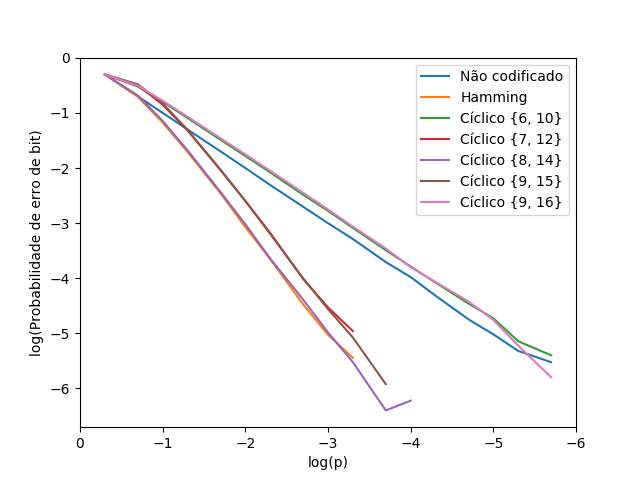
\includegraphics[scale=0.6]{floats/cyclic_5x10e6.png}
	\caption{\label{fig:cyclic_comparison}Comparação da eficácia dos códigos cíclicos para 5004720 bits de informação enviados.}
\end{figure}

A título de comparação, a Figura \ref{fig:non_cyclic_comparison} traz os resultados do experimento anterior, o qual empregou códigos não necessariamente cíclicos obtidos pela tentativa de maximizar a distância mínima por meio de incrementos no tamanho de bloco.

\begin{figure}[!hb]
	\centering
	\captionsetup{justification=centering}
	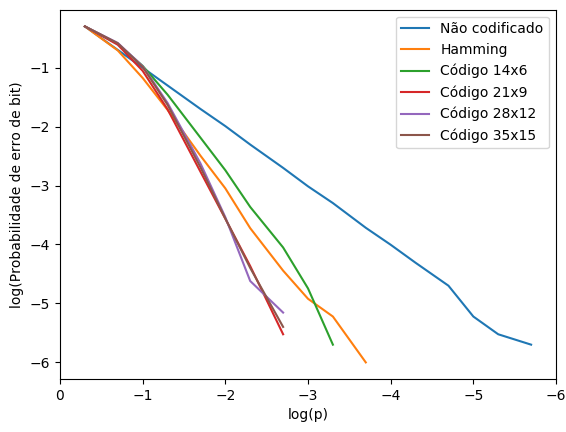
\includegraphics[scale=0.45]{floats/non_cyclic.png}
	\caption{\label{fig:non_cyclic_comparison}Comparação da eficácia dos códigos não necessariamente cíclicos para 1000080 bits de informação enviados.}
\end{figure}

\subsection{Códigos BCH}

\subsubsection{\label{complexidade_decod}Complexidade de decodificação BCH}

Segundo \cite{ref:algoritmo-berlekamp}, a decodificação de códigos BCH se dá em $\mathcal{O}(n)$, $n$ sendo o tamanho de bloco empregado. Para confirmar a validade dessa afirmação, construíram-se códigos $BCH(m, 3)$, com $m \in \lbrace 4,5,...,20 \rbrace$, e mediram-se os tempos de decodificação submetendo a mesma palavra a cada um deles, com resultados ilustrados pela Figura \ref{fig:bch_decoding_is_linear}.

\begin{figure}[!hb]
	\centering
    \captionsetup{justification=centering}
	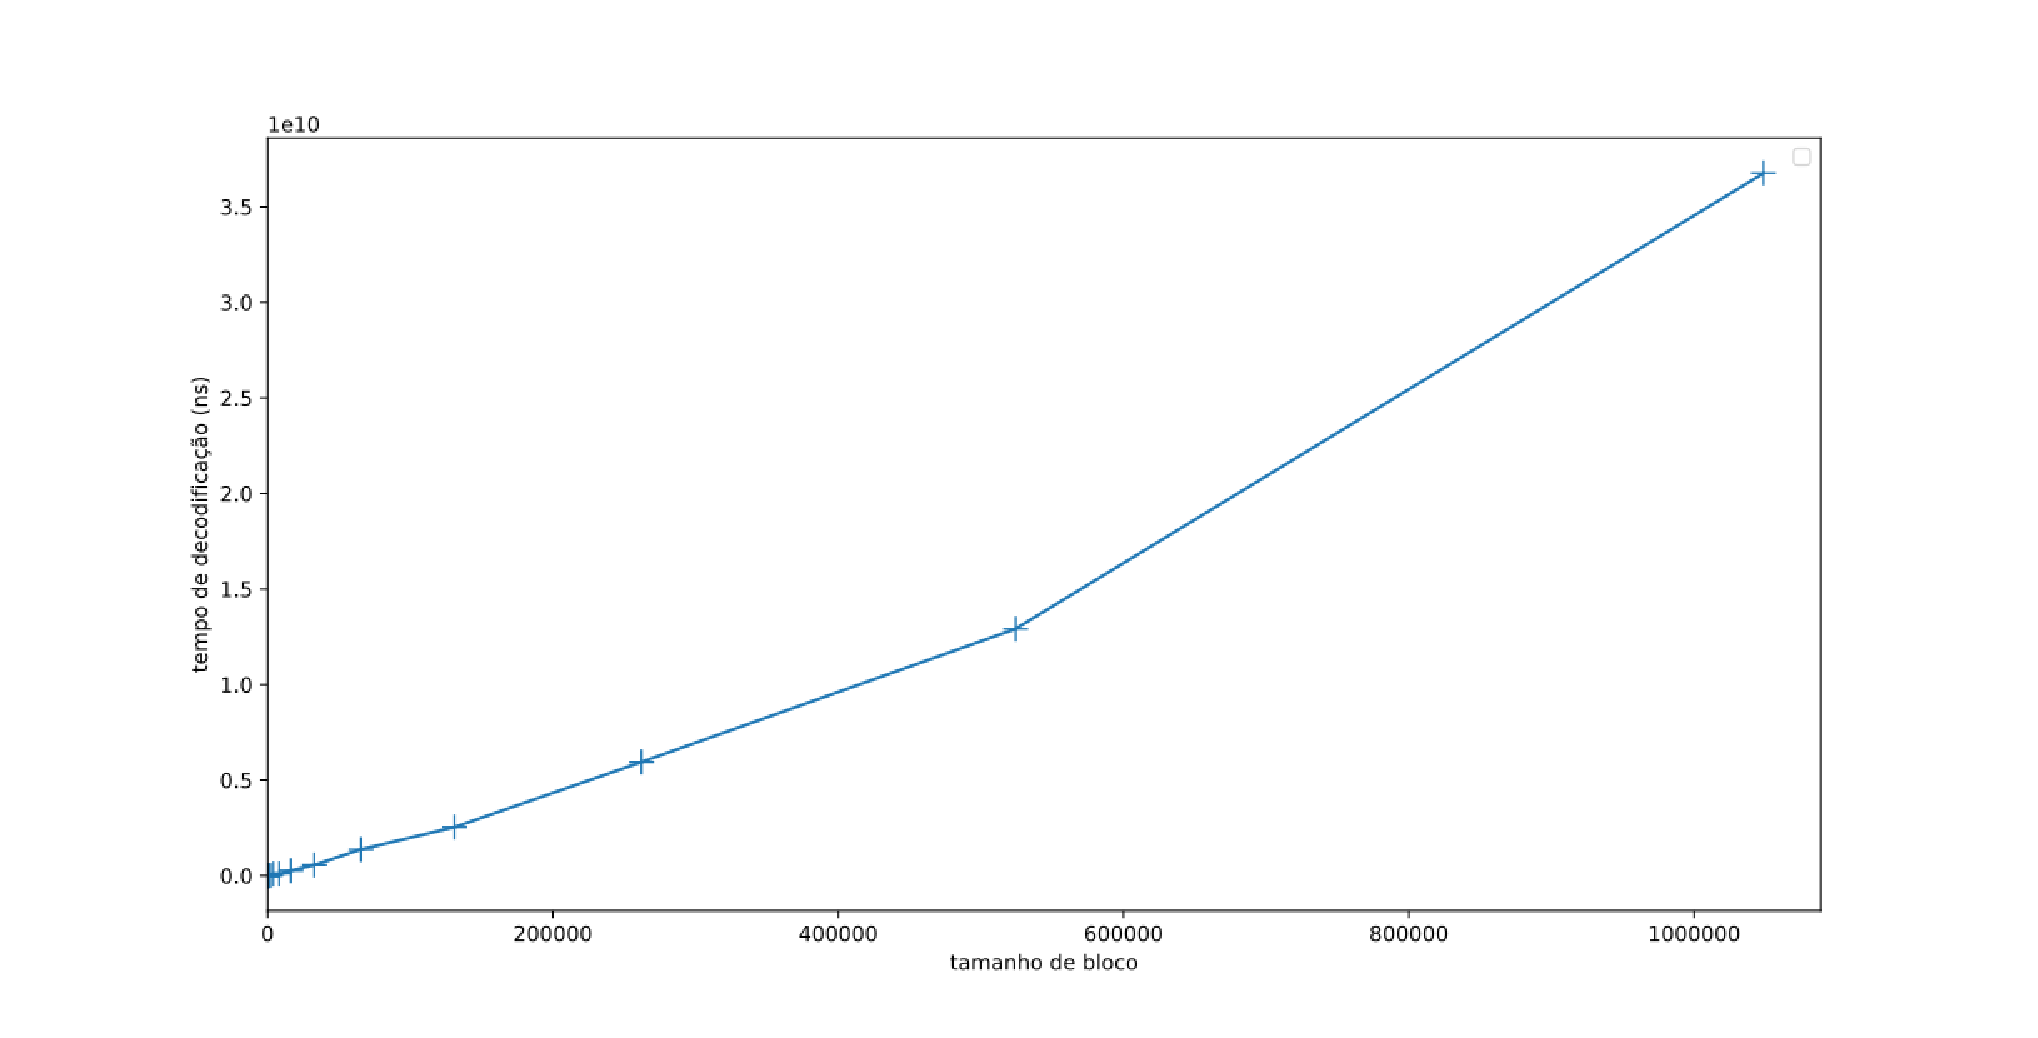
\includegraphics[scale=0.3]{floats/bch-decode-is-linear.eps}
	\caption{\label{fig:bch_decoding_is_linear}Tempo de decodificação para BCH com variados tamanhos de bloco.}
\end{figure}

\subsubsection{\label{desempenho_bch}Desempenho do BCH}

Para comparar o código BCH aos outros cíclicos, procurou-se um BCH de taxa próxima a 4/7 (usada como referência nos outros códigos deste laboratório), elegendo-se $BCH(5, 3)$ para ser submetido a testes sob canal BSC. A escolha se deu com base no polinômio gerador calculado, $g(X)=X^{15}+X^{11}+X^{10}+X^9+X^8+X^7+X^5+X^3+X^2+X+1$, que rendeu ao código taxa $\frac{31-15}{31}\simeq 0.52\simeq \frac{4}{7}\simeq 0.57$.

Somente pela superior distância mínima projetada (3), era de se esperar que $BCH(5,3)$ superasse todos os outros códigos descritos neste texto. Isso é corroborado pela Figura \ref{fig:bch_performance}, na qual se vê que ele supera $Hamming(4,7)$ (que, por sua vez, tinha o mesmo desempenho aproximado dos outros códigos cíclicos).

\begin{figure}[!hb]
	\centering
    \captionsetup{justification=centering}
	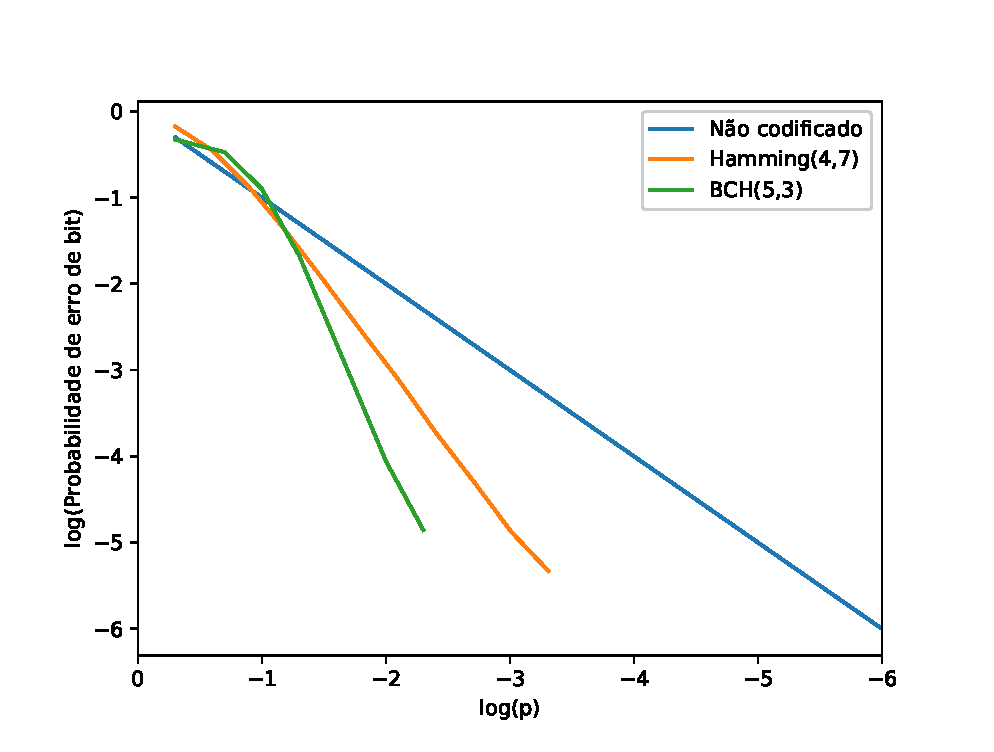
\includegraphics[scale=0.6]{floats/bch-performance.eps}
	\caption{\label{fig:bch_performance}Chances de erro de bit de informação para $BCH(5,3)$ e $Hamming(4,7)$ sujeitos a canais BSC de variadas taxas de erro de bit.}
\end{figure}

\section{Conclusão}
 O código cíclico apresenta a vantagem de ser necessário armazenar uma quantidade menor de síndromes e de não ser necessário associar síndrome a erro na decodificação. Isso introduz maior complexidade no passo de decodificação pois não há mapeamento direto entre síndrome e erro. No entanto, no código desenvolvido pelas equipes, foi necessário criar um método para geração de códigos. Dessa forma a complexidade do desenvolvimento do código cíclico é maior no tocante ao entendimento dos conceitos envolvidos e no código do experimento anterior no tocante à criação de um procedimento para a geração da matriz de paridade.
 
 Pôde-se notar do gráfico presente em Figura \ref{fig:cyclic_comparison} que o código de Hamming é mais eficiente que quase todos os códigos implementados, com exceção do BCH. Isso era esperado uma vez que nenhum dos outros códigos cíclicos corrige mais bits que Hamming e Hamming possui bloco menor que os demais. Nota-se que os casos de distância mínima dois são ligeiramente piores que o canal não codificado e que o caso de distância mínima três é muito próximo de Hamming.
 
 Pode-se depreender que os códigos cíclicos, da maneira como foram desenvolvidos, são ineficazes na diminuição da distância mínima com o aumento do tamanho do bloco. Em contraste a isso, os códigos do experimento anterior apresentados na Figura \ref{fig:non_cyclic_comparison} são, em sua maioria, mais eficazes que Hamming.
 
 Os tamanhos de códigos cíclicos utilizados variaram de 10 ao maior tamanho requisitado (16) e o método utilizado para gerar o conjunto de síndromes é extensível para tamanhos maiores de códigos. Vale notar que a etapa crítica de geração do conjunto de síndromes só precisa ser realizada uma única vez no preprocessamento, por isso, seu tempo de execução total não é crítico.
 
 A medida entre tamanho do bloco e desempenho é dada pela complexidade da multiplicação e divisão polinomial, nesse caso foram consideradas ambas $\mathcal{O}(n^2)$. Além disso, foram discutidos mais detalhes sobre as complexidades das implementações na explicação do algoritmo.

 Por outro lado, o código BCH possui rica estrutura matemática subjacente (corpos), possibilitando completa flexibilidade para gerar tamanhos de bloco arbitrariamente grandes e distâncias mínimas desejadas. Além de ser robusto por construção, ainda se caracteriza por complexidade linear de decodificação, como foi empiricamente validado.

\begin{thebibliography}{1}

\bibitem{ref:algoritmo-berlekamp}
Berlekamp, Elwyn R. \emph{Algebraic Coding Theory}. Edição revisada. Singapura: WSPC, 2015. 
\bibitem{ref:roteiro}
Sharma, Manish \emph{Aula2 - Códigos Cíclicos}. ELE32-Introdução a Comunicações. 2018. 

\end{thebibliography}

\end{document}
